\documentclass{article}

\usepackage[english, russian]{babel}
\usepackage{geometry}
\usepackage{graphicx}
\usepackage{listings}
\usepackage{xcolor}

\lstdefinestyle{asm}{
	language={[x86masm]Assembler},
	basicstyle=\footnotesize\ttfamily,
	commentstyle=\color{gray},
	numbers=left,
	frame=single,
	tabsize=4,
	breaklines=true
}

\lstset{
	literate=
	{а}{{\selectfont\char224}}1
	{б}{{\selectfont\char225}}1
	{в}{{\selectfont\char226}}1
	{г}{{\selectfont\char227}}1
	{д}{{\selectfont\char228}}1
	{е}{{\selectfont\char229}}1
	{ё}{{\"e}}1
	{ж}{{\selectfont\char230}}1
	{з}{{\selectfont\char231}}1
	{и}{{\selectfont\char232}}1
	{й}{{\selectfont\char233}}1
	{к}{{\selectfont\char234}}1
	{л}{{\selectfont\char235}}1
	{м}{{\selectfont\char236}}1
	{н}{{\selectfont\char237}}1
	{о}{{\selectfont\char238}}1
	{п}{{\selectfont\char239}}1
	{р}{{\selectfont\char240}}1
	{с}{{\selectfont\char241}}1
	{т}{{\selectfont\char242}}1
	{у}{{\selectfont\char243}}1
	{ф}{{\selectfont\char244}}1
	{х}{{\selectfont\char245}}1
	{ц}{{\selectfont\char246}}1
	{ч}{{\selectfont\char247}}1
	{ш}{{\selectfont\char248}}1
	{щ}{{\selectfont\char249}}1
	{ъ}{{\selectfont\char250}}1
	{ы}{{\selectfont\char251}}1
	{ь}{{\selectfont\char252}}1
	{э}{{\selectfont\char253}}1
	{ю}{{\selectfont\char254}}1
	{я}{{\selectfont\char255}}1
	{А}{{\selectfont\char192}}1
	{Б}{{\selectfont\char193}}1
	{В}{{\selectfont\char194}}1
	{Г}{{\selectfont\char195}}1
	{Д}{{\selectfont\char196}}1
	{Е}{{\selectfont\char197}}1
	{Ё}{{\"E}}1
	{Ж}{{\selectfont\char198}}1
	{З}{{\selectfont\char199}}1
	{И}{{\selectfont\char200}}1
	{Й}{{\selectfont\char201}}1
	{К}{{\selectfont\char202}}1
	{Л}{{\selectfont\char203}}1
	{М}{{\selectfont\char204}}1
	{Н}{{\selectfont\char205}}1
	{О}{{\selectfont\char206}}1
	{П}{{\selectfont\char207}}1
	{Р}{{\selectfont\char208}}1
	{С}{{\selectfont\char209}}1
	{Т}{{\selectfont\char210}}1
	{У}{{\selectfont\char211}}1
	{Ф}{{\selectfont\char212}}1
	{Х}{{\selectfont\char213}}1
	{Ц}{{\selectfont\char214}}1
	{Ч}{{\selectfont\char215}}1
	{Ш}{{\selectfont\char216}}1
	{Щ}{{\selectfont\char217}}1
	{Ъ}{{\selectfont\char218}}1
	{Ы}{{\selectfont\char219}}1
	{Ь}{{\selectfont\char220}}1
	{Э}{{\selectfont\char221}}1
	{Ю}{{\selectfont\char222}}1
	{Я}{{\selectfont\char223}}1
}

\geometry{pdftex, left = 3cm, right = 1cm, top = 2cm, bottom = 2cm}

\begin{document}
\begin{titlepage}
	\noindent\begin{tabular}{|c|c|}	\hline
	\noindent\begin{minipage}{0.14\textwidth}
		
\includegraphics[width=\linewidth]{tools/logo.png}
	\end{minipage} &
	\noindent\begin{minipage}{0.75\textwidth}\centering
		\textbf{\newline Министерство науки и высшего образования Российской Федерации}\\
		\textbf{Федеральное государственное бюджетное образовательное учреждение высшего образования}\\
		\textbf{«Московский государственный технический университет имени Н.Э.~Баумана}\\
		\textbf{(национальный исследовательский университет)»}\\
		\textbf{(МГТУ им. Н.Э.~Баумана)}
	\end{minipage} \\
	\hline	\end{tabular}\newline\newline\newline\newline
	\noindent ФАКУЛЬТЕТ \underline{«Информатика и системы управления»} \newline\newline
	\noindent КАФЕДРА \underline{«Программное обеспечение ЭВМ и информационные технологии»}\newline\newline\newline\newline\newline\newline\newline\newline\newline

	\noindent\begin{minipage}{1.0\textwidth}\centering
		\Large\textbf{   ~~~ Лабораторная работа №1}\newline
		\textbf{по дисциплине "Операционные системы"}\newline\newline\newline\newline\newline\newline\newline\newline
	\end{minipage}

	\noindent\textbf{Тема} \underline{Дизассемблирование INT 8h}\newline\newline
	\textbf{Студент} \underline{Тузов Даниил Александрович}\newline\newline
	\textbf{Группа} \underline{ИУ7-52Б}\newline\newline
	\textbf{Преподаватель} \underline{Рязанова Наталья Юрьевна}
	
	\begin{center}
		\vfill
		Москва, \the\year ~г.
	\end{center}
	\clearpage
\end{titlepage}

\section{Дизассемблированные коды}
\subsection{Дизассемблированный код обработчика прерывания int8h}
\begin{lstlisting}[style={asm}]
            Temp.lst				Sourcer	v5.10   18-Sep-24  12:41 am   Page 1

; Вызов сабрутины
020C:0746  E8 0070				call	sub_1			; (07B9)
020C:0746  E8 70 00				db	0E8h, 70h, 00h
; Сохранение регистров
020C:0749  06					push	es
020C:074A  1E					push	ds
020C:074B  50					push	ax
020C:074C  52					push	dx
; Записать в DS - 40h 
020C:074D  B8 0040				mov	ax,40h
020C:0750  8E D8				mov	ds,ax
; Записать в ES - 00h
020C:0752  33 C0				xor	ax,ax			; Zero register
020C:0754  8E C0				mov	es,ax
; Инкремент младшего слова счетчика тиков
020C:0756  FF 06 006C				inc	word ptr ds:[6Ch]	; (0040:006C=0B1F0h)
020C:075A  75 04				jnz	loc_1			; Jump if not zero
; Инкремент старшего слова тиков, если обнулилось младшее
020C:075C  FF 06 006E				inc	word ptr ds:[6Eh]	; (0040:006E=0)
020C:0760			loc_1:
; Если старшее слово равно 24 и младшее равно 176, значит прошел день и надо сбросить счетчики
020C:0760  83 3E 006E 18			cmp	word ptr ds:[6Eh],18h	; (0040:006E=0)
020C:0765  75 15				jne	loc_2			; Jump if not equal
020C:0767  81 3E 006C 00B0			cmp	word ptr ds:[6Ch],0B0h	; (0040:006C=0B1F0h)
020C:076D  75 0D				jne	loc_2			; Jump if not equal
; Сброс младшего слова
020C:076F  A3 006E				mov	word ptr ds:[6Eh],ax	; (0040:006E=0)
; Сброс старшего слова
020C:0772  A3 006C				mov	word ptr ds:[6Ch],ax	; (0040:006C=0B1F0h)
; Занесение значения 1 в ds:[70h]
020C:0775  C6 06 0070 01			mov	byte ptr ds:[70h],1	; (0040:0070=0)
; Установка 3-его бита в al
020C:077A  0C 08				or	al,8
020C:077C			loc_2:
020C:077C  50					push	ax
;Декремент счетчика времени до отключения моторчика дисковода
020C:077D  FE 0E 0040				dec	byte ptr ds:[40h]	; (0040:0040=94h)
020C:0781  75 0B				jnz	loc_3			; Jump if not zero
; Если счетчик обнулился, сбрасывается флаг работы моторчика
020C:0783  80 26 003F F0			and	byte ptr ds:[3Fh],0F0h	; (0040:003F=0)
;Отправка команды 0Ch отключения моторчика дисковода на порт 3F2h
020C:0788  B0 0C				mov	al,0Ch
020C:078A  BA 03F2				mov	dx,3F2h
020C:078D  EE					out	dx,al			; port 3F2h, dsk0 contrl output
020C:078E			loc_3:
020C:078E  58					pop	ax
; Проверка флага четности
020C:078F  F7 06 0314 0004			test	word ptr ds:[314h],4	; (0040:0314=3200h)
020C:0795  75 0C				jnz	loc_4			; Jump if not zero
; Загрузка младшего байта регистра флагов в ah
020C:0797  9F					lahf				; Load ah from flags
020C:0798  86 E0				xchg	ah,al
020C:079A  50					push	ax
; Косвенный вызов прерывания 1Ch
020C:079B  26: FF 1E 0070			call	dword ptr es:[70h]	; (0000:0070=6ADh)
020C:07A0  EB 03				jmp	short loc_5		; (07A5)
020C:07A2  90					nop
020C:07A3			loc_4:
; Вызов прерывания 1Ch
020C:07A3  CD 1C				int	1Ch			; Timer break (call each 18.2ms)
020C:07A5			loc_5:
; Вызов сабрутины
020C:07A5  E8 0011				call	sub_1			; (07B9)
; Сброс контроллера прерываний (разрешаются прерывания с более низким приоритетом)
020C:07A8  B0 20				mov	al,20h			; ' '
020C:07AA  E6 20				out	20h,al			; port 20h, 8259-1 int command
										;  al = 20h, end of interrupt
; Восстановление регистров
020C:07AC  5A					pop	dx
020C:07AD  58					pop	ax
020C:07AE  1F					pop	ds
020C:07AF  07					pop	es
020C:07B0  E9 FE99				jmp	$-164h
; ...
020C:06AC CF					itret			; Возврат из прерывания
\end{lstlisting}

\subsection{Дизассемблированный код subrouting}
\begin{lstlisting}[style={asm}]
				sub_1		proc	near
; Сохранение значений регистров
020C:07B9  1E					push	ds
020C:07BA  50					push	ax
; Записать в DS - 40h 
020C:07BB  B8 0040				mov	ax,40h
020C:07BE  8E D8				mov	ds,ax
; Загрузка младшего байта регистра флагов в ah
020C:07C0  9F					lahf				; Load ah from flags
; Проверка флага DF и старшего бита флага IOPL
020C:07C1  F7 06 0314 2400			test	word ptr ds:[314h],2400h	; (0040:0314=3200h)
020C:07C7  75 0C				jnz	loc_7			; Jump if not zero
; Сброс флага прерываний IF
020C:07C9  F0> 81 26 0314 FDFF	                           lock	and	word ptr ds:[314h],0FDFFh	; (0040:0314=3200h)
020C:07D0			loc_6:
; Загрузка из ah младшего байта регистра флагов
020C:07D0  9E					sahf				; Store ah into flags
; Восстановление регистров
020C:07D1  58					pop	ax
020C:07D2  1F					pop	ds
020C:07D3  EB 03				jmp	short loc_8		; (07D8)
020C:07D5			loc_7:
; Сброс флага прерываний IF
020C:07D5  FA					cli				; Disable interrupts
020C:07D6  EB F8				jmp	short loc_6		; (07D0)
020C:07D8			loc_8:
020C:07D8  C3					retn
				sub_1		endp
\end{lstlisting}

\section{Схемы алгоритмов}
\subsection{Схема алгоритма обработчика прерывания int8h}
\begin{center}
	\noindent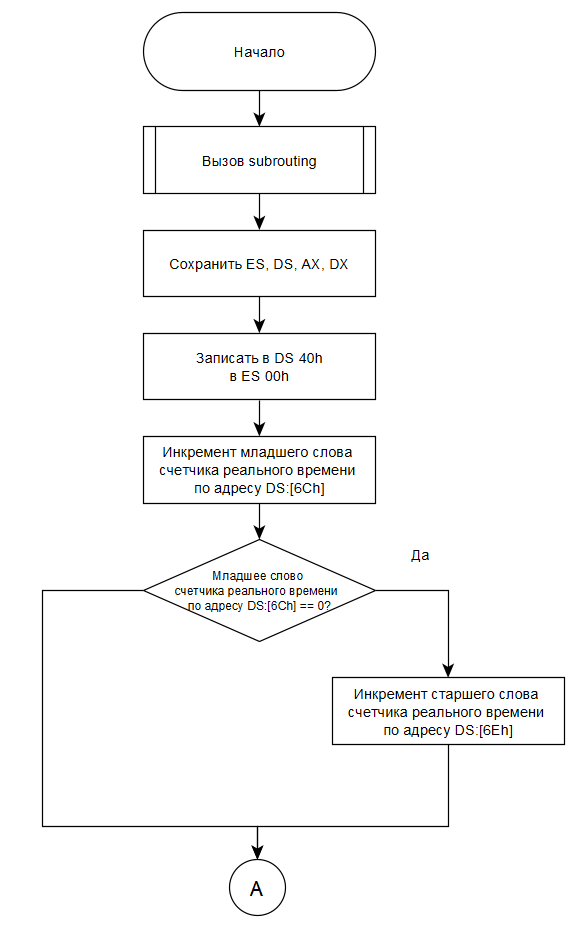
\includegraphics{tools/Screenshot_5.png}
	\clearpage
	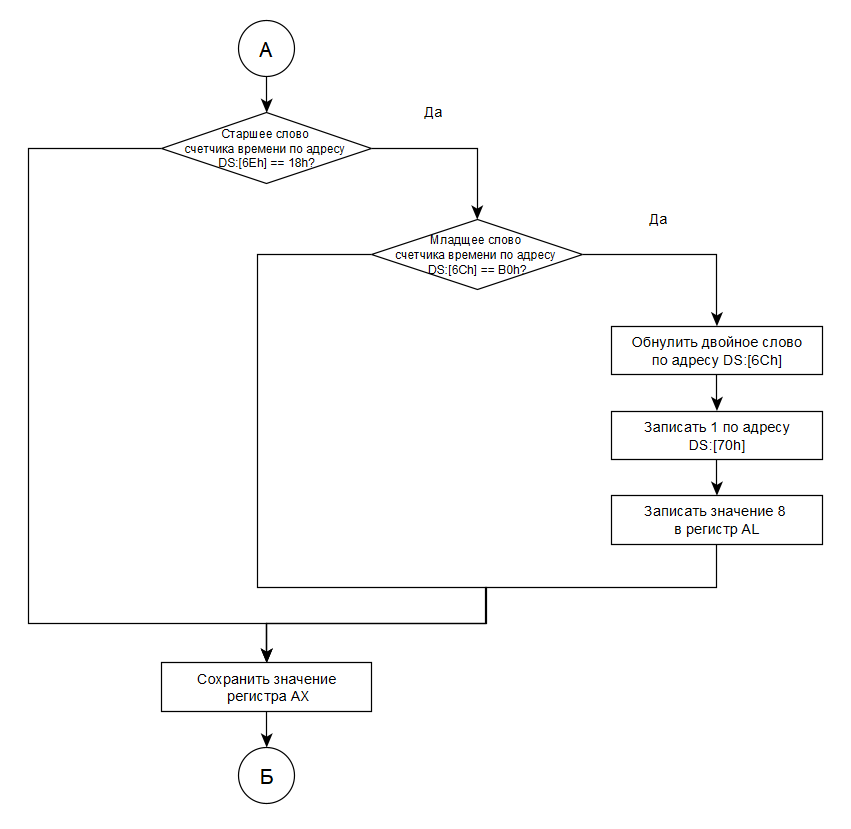
\includegraphics{tools/Screenshot_4.png}
	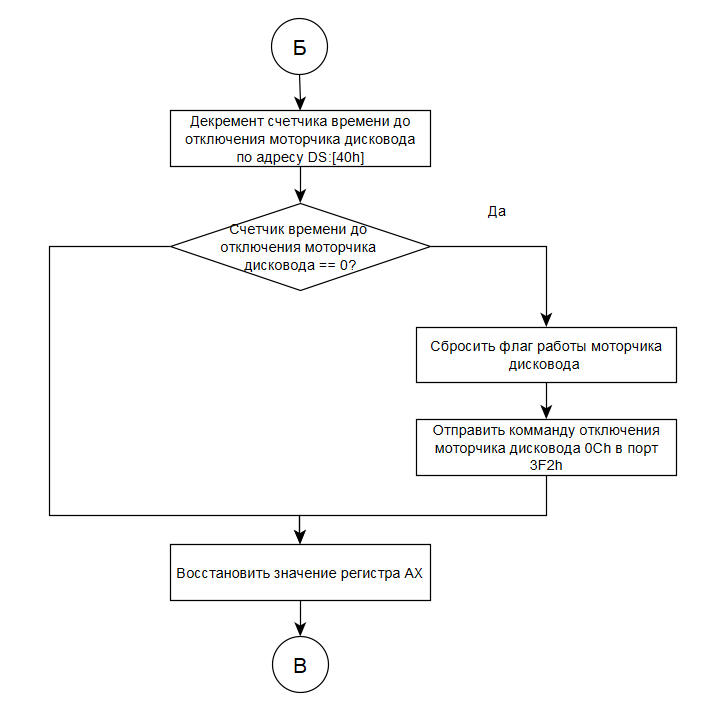
\includegraphics{tools/Screenshot_3.png}
	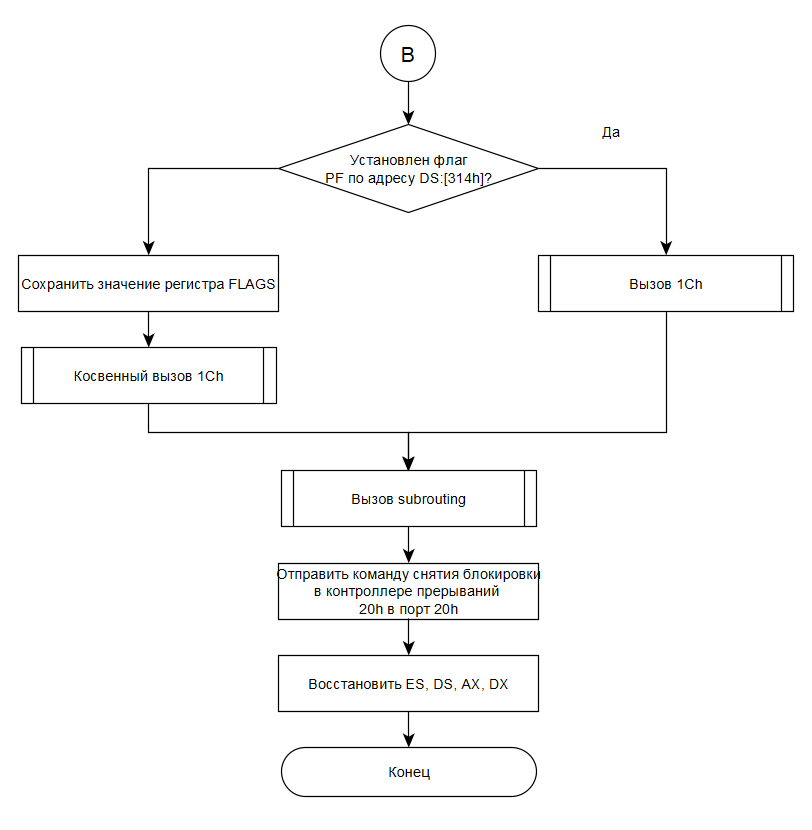
\includegraphics{tools/Screenshot_2.png}
\end{center}
\subsection{Схема алгоритма subrouting}

\begin{center}
	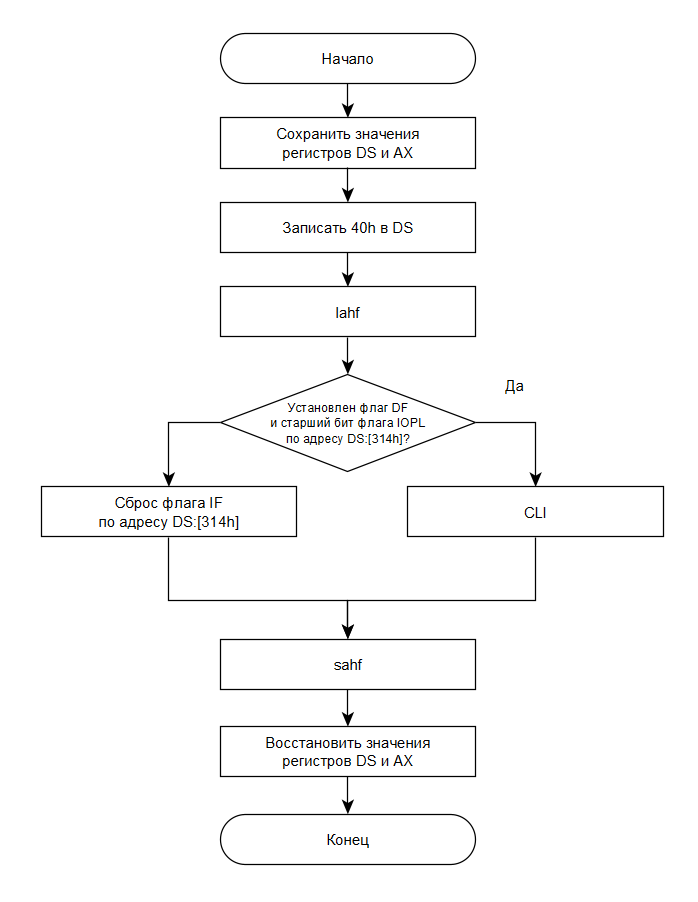
\includegraphics[height=0.98\textheight]{tools/Screenshot_1.png}
\end{center}

\end{document}